\documentclass{article}
\usepackage[utf8]{inputenc}
\usepackage[margin=1in]{geometry} % Ajusta los márgenes a 1 pulgada
\usepackage{graphicx}
\usepackage{listings}
\usepackage{xcolor}
\usepackage{hyperref}
\usepackage{tikz}
\usepackage{biblatex}
\usepackage{lstmisc}
\usetikzlibrary{shapes.multipart}

\definecolor{codegreen}{rgb}{0,0.6,0}
\definecolor{codegray}{rgb}{0.5,0.5,0.5}
\definecolor{codepurple}{rgb}{0.58,0,0.82}
\definecolor{backcolour}{rgb}{0.95,0.95,0.92}

\lstdefinestyle{mystyle}{
    backgroundcolor=\color{backcolour},
    commentstyle=\color{codegreen},
    keywordstyle=\color{magenta},
    numberstyle=\tiny\color{codegray},
    stringstyle=\color{codepurple},
    basicstyle=\ttfamily\small,
    breakatwhitespace=false,
    breaklines=true,
    captionpos=b,
    keepspaces=true,
    numbers=left,
    numbersep=5pt,
    showspaces=false,
    showstringspaces=false,
    showtabs=false,
    tabsize=2
}

\lstset{style=mystyle}

\title{Convolutional Neural Networks – Lab 4}
\author{RUBEN MARTINEZ GONZALEZ}
\date{Marzo 2024}

\begin{document}

    \maketitle


    \section{introducción}\label{sec:introduccion}
    En este informe, se presenta el trabajo realizado en el laboratorio 4 de Redes Neuronales Convolucionales.
    El objetivo principal es implementar una red neuronal (NN) artificial multiclase de retropropagación para clasificar las imágenes de dígitos del 0 al 9 escritos a mano.
    \newline
    Se utilizará las imágenes de la base de datos mnist.txt, se entrenara la NN utilizando las primeras 900 imágenes y se probara con las 100 restantes.
    Se calculará el error de la función de costo para cada época.
    Se presentarán datos del entrenamiento, resultados y comentarios.

    \noindent
    La solución se implementó en Python utilizando la biblioteca NumPy para el procesamiento de matrices,
    Matplotlib para la visualización de gráficos y Scikit-learn solo para la separación de los datos en conjuntos de entrenamiento y prueba.
    \newline
    La implementación está desplegada en un notebook de Google Colab, el cual se puede acceder a través del siguiente enlace:
    \texttt{%
        \href{https://drive.google.com/file/d/1G7FsF-o0YyQpEuUWFcWKjgZJbzFlSa0B/view?usp=sharing}{%
            Colab}%
    }


    \section{Procesamiento de datos}\label{sec:Procesamiento-de-datos}

    \subsection{Descripción}\label{subsec:descripcion}
    El procesamiento realizado para interpretar y segmentar los datos de la base de datos de mnist.txt se describe a continuación:
    \begin{itemize}
        \item Se lee el archivo mnist.txt y se invoca la función load\_data para cargar los datos en memoria.
        \item La función load\_data recibe como parámetro la ruta del archivo y retorna dos listas, una con las características de las imágenes y otra con las etiquetas de las imágenes.
        \item La función load\_data extrae las características de todos los primeros 784 valores de cada renglón y las etiquetas del último valor de cada renglón.
        \item Para visualizar una imagen aleatoria de los datos extraídos de mnist.txt se genera un índice aleatorio
        y se invoca la función visualize\_image pasando como parámetros las características (784 píxeles) y la etiqueta de la imagen correspondiente al índice aleatorio.
        \item Luego se visualiza la imagen en una matriz de 28x28 píxeles y se muestra la etiqueta correspondiente.
        \item Finalmente, se separan los datos en dos conjuntos, uno de entrenamiento y otro de prueba, utilizando la función train\_test\_split de la biblioteca scikit-learn.
        \item La separación de datos se realiza de un total de 1000 imágenes, 900 para entrenamiento (90\%) y 100 para prueba (10\%).
    \end{itemize}

    \subsection{Implementación}\label{subsec:implementacion}

    \begin{lstlisting}[language=Python, caption={carga de datos}, label={lst:load_data}]
def load_data(file_path):
    with open(file_path) as file:
        data = [line.strip().split(" ") for line in file]
        features = [np.asarray(data_point[:784], dtype=float) for data_point in data] # pixeles de la imágen
        labels = [float(data_point[-1]) for data_point in data]                       # clase a la que pertenece
    return features, labels
# Cargar los datos
file_path = "mnist.txt"
images, labels = load_data(file_path)
    \end{lstlisting}

    \begin{lstlisting}[language=Python, caption={Visualización de datos}, label={lst:visualize_data}]
def visualize_image(images, labels, n):
    if n >= len(images):
        print("El índice n está fuera del rango.")
        return
    image = images[n].reshape(28, 28)  # reconstruye la imagen en matriz de 28x28
    label = int(labels[n])

    plt.imshow(image, cmap='gray')
    plt.title(f"Imagen del dígito: {label} índice:{n}")
    plt.axis('off')
    plt.show()
# Visualizar la imagen en la posición n
import random
n = random.randint(0, 5000)
visualize_image(images, labels, n)
    \end{lstlisting}

    \noindent
    Separación de datos en conjuntos de entrenamiento y prueba:
    \begin{lstlisting}[language=Python, caption={Separación de datos}, label={lst:split_data}]
X_train, X_test, Y_train, Y_test = train_test_split(np.asarray(images[:1000]), labels[:1000], test_size=0.1, shuffle=True)
    \end{lstlisting}

    \clearpage
    \noindent
    Al ejecutar el código se obtuvo la siguiente gráfica:
    \begin{figure}[h]
        \centering
        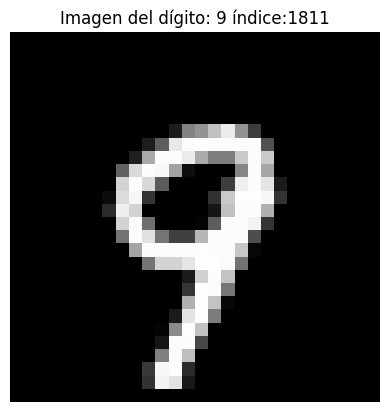
\includegraphics[width=0.5\textwidth]{img/ramdom_mnist}
        \caption{Gráfica de los datos de entrenamiento}
        \label{fig:random_mnist}
    \end{figure}

    \clearpage


    \section{Descripción del problema}\label{sec:descripcion-del-problema}
    A partir de las imágenes (28 x 28) extraídas de la base de datos mnist.txt de dígitos del 0 al 9 escritos a mano y sus correspondientes etiquetas,
    se busca entrenar una red neuronal artificial para clasificar las imágenes en las 10 clases correspondientes a los dígitos del 0 al 9.
    El objetivo es implementar una red neuronal artificial multiclase de retropropagación para clasificar estas imágenes.


    \section{Método utilizado}\label{sec:metodo-utilizado}
    La solución propuesta para el problema de clasificación de imágenes de dígitos escritos a mano se implementó utilizando una red neuronal(NN) de retropropagación que se describe a continuación:
    \begin{itemize}
        \item La red neuronal implementada consta de 3 capas, una capa de entrada, una capa oculta y una capa de salida.
        \item La capa de entrada consta de 784 neuronas, una por cada pixel de la imagen.
        \item La capa oculta consta de 300 neuronas y la capa de salida consta de 10 neuronas, una por cada clase.
        \item La función de activación utilizada para las neuronas de la capa oculta es la función de activación sigmoide.
        \item La taza de aprendizaje utilizada es de 0.001 y el número de épocas es de 400.
        \item La función de costo utilizada es la entropía cruzada.
        \item La actualización de los pesos se realiza utilizando el algoritmo de retropropagación con descenso del gradiente.
        \item La red neuronal implementada consta de 3 métodos principales, el método forward\_propagation, el método backward\_propagation y el método train.
        \item El método forward\_propagation se encarga de realizar la propagación hacia adelante de las activaciones de las neuronas de la red.
        \item El método backward\_propagation se encarga de realizar la propagación hacia atrás de los gradientes de las neuronas de la red.
        \item El método train se encarga de entrenar la red neuronal utilizando los datos de entrenamiento y retorna el historial de la pérdida en cada época.
        \item El método predict se encarga de realizar la predicción de las clases de las imágenes según la red neuronal entrenada.
    \end{itemize}
    \clearpage

    \subsection{Gráfica de la estructura de la red neuronal}\label{subsec:grafica-de-la-estructura-de-la-red-neuronal}
    \begin{figure}[h]
        \centering
        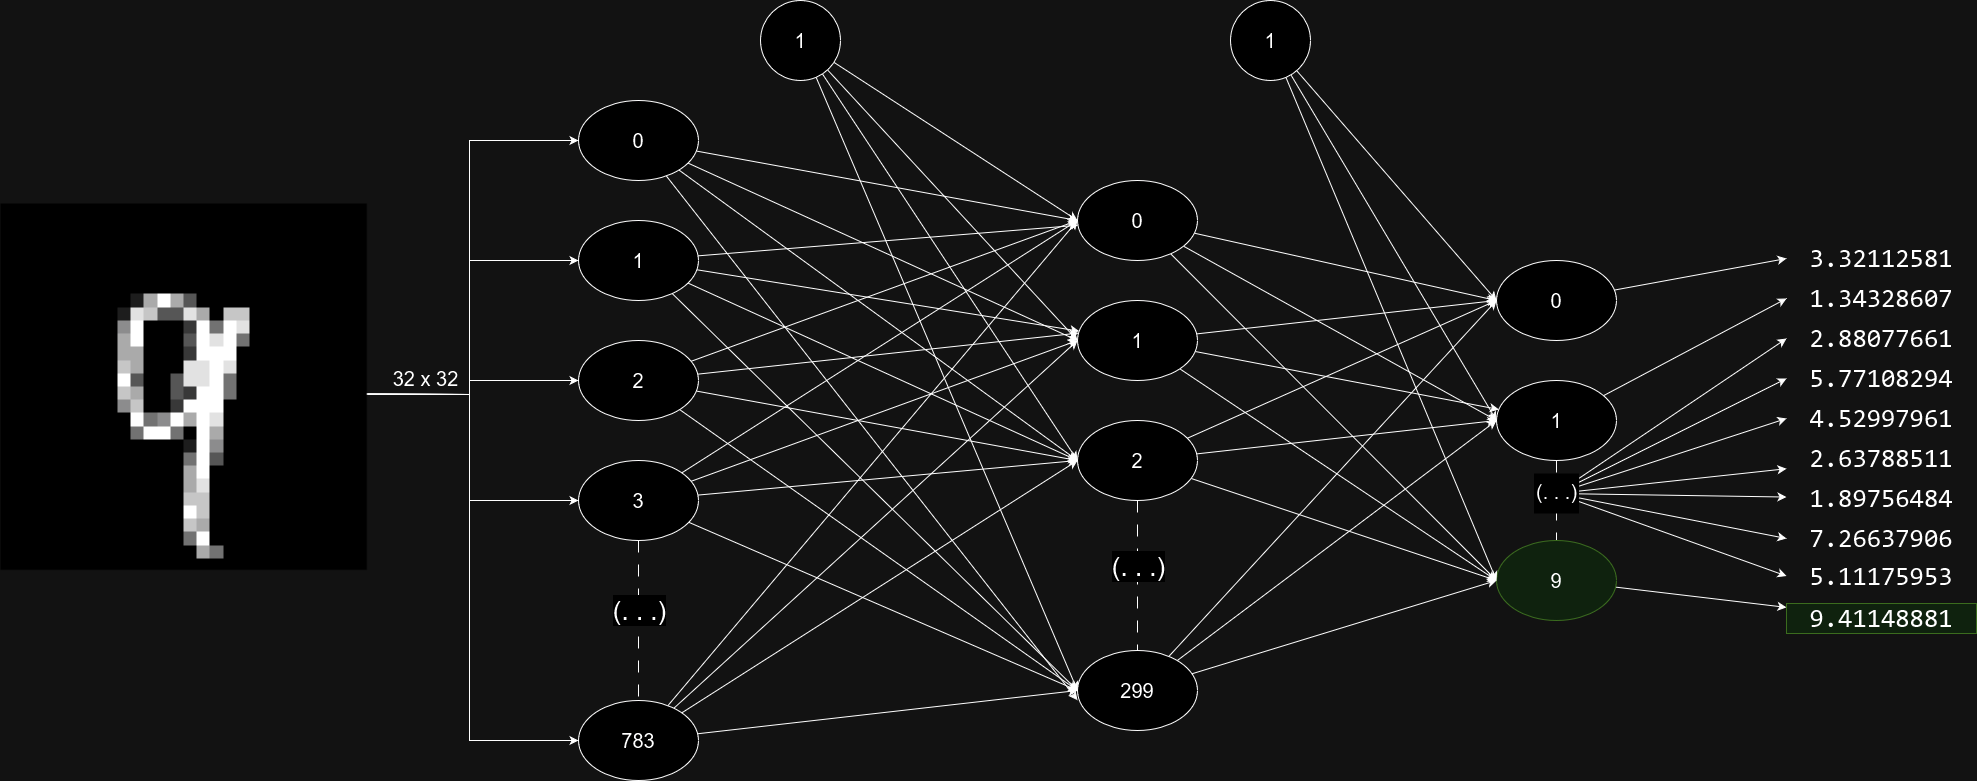
\includegraphics[width=0.99\textwidth]{img/red}
        \caption{Gráfica de la estructura de la red neuronal}
        \label{fig:red_neuronal}
    \end{figure}

    \section{Entrenamiento de la red neuronal}\label{sec:entrenamiento-de-la-red-neuronal}

    \subsection{función de costo}\label{subsec:funcion-de-costo}

    Como función de costo se utilizó la función de costo de entropía cruzada, la cual se define como:
    \begin{equation}
        J(\theta) = -\frac{1}{m} \sum_{i=1}^{m} y^{(i)} \log(h_{\theta}(x^{(i)})) + (1 - y^{(i)}) \log(1 - h_{\theta}(x^{(i)}))\label{eq:equation}
    \end{equation}
    Como derivada de la función de costo de entropía cruzada se utilizó la siguiente expresión:
    \begin{equation}
        \frac{\partial J(\theta)}{\partial \theta} = -\frac{y}{h_{\theta}(x)} + \frac{1 - y}{1 - h_{\theta}(x)}\label{eq:equation2}
    \end{equation}
    Para la implementación de la función de costo se creó una clase llamada CrossEntropy la cual garantiza la regresión logística.
    Con un método principal al invocar la clase que recibe como parámetros las predicciones y las etiquetas y retorna el valor de la función de costo.
    Además, se implementó un método derivado que recibe como parámetros las predicciones y las etiquetas y retorna el valor de la derivada de la función de costo.
    Para los cálculos con epsilon se utilizó un valor pequeño definido como 1e-10 para evitar errores matemáticos.

    \begin{lstlisting}[language=Python, caption={Función de costo}, label={lst:cost_function}]
class CrossEntropy:
    def __init__(self, epsilon=1e-10):# Valor pequeño para evitar errores matemáticos
        self.epsilon = epsilon

    def __call__(self, P, Y): # Función de costo de entropía cruzada
        return -np.mean(Y * np.log(P + self.epsilon) + (1 - Y) * np.log(1 - P + self.epsilon))

    def derivative(self, P, Y):
        return -(Y / (P + self.epsilon)) + (1 - Y) / (1 - P + self.epsilon)
    \end{lstlisting}

    \subsection{Función de activación}\label{subsec:funcion-de-activacion}

    Como función de activación se utilizó la función sigmoide, la cual se define como:
    \begin{equation}
        \sigma(x) = \frac{1}{1 + e^{-x}}\label{eq:equation3}
    \end{equation}
    Como derivada de la función de activación sigmoide se utilizó la siguiente expresión:
    \begin{equation}
        \sigma'(x) = \sigma(x)(1 - \sigma(x))\label{eq:equation4}
    \end{equation}
    \noindent
    Para la implementación de la función de activación sigmoide se creó una clase llamada Sigmoid
    la cual será utilizada para la activación de las neuronas.
    Esta clase tiene un método principal que recibe como parámetro un valor x, y retorna el valor de la función sigmoide.
    Además, se implementó un método derivado que recibe como parámetro un valor x, y retorna el valor de la derivada de la función sigmoide.

    \begin{lstlisting}[language=Python, caption={Función de activación}, label={lst:activation_function}]
class Sigmoid: # Sigmoid Activation function
    def __call__(self, x):
    return 1 / (1 + np.e ** (-x))

    def derivative(self, x):
    return x * (1 - x)
    \end{lstlisting}

    \subsection{Capas de la red neuronal}\label{subsec:capas-de-la-red-neuronal}
    Para la implementación de las capas de la red neuronal se creó una clase llamada Layer
    la cual será utilizada para instanciar las capas de la red.
    El constructor de la clase recibe como parámetros el número de conexiones y el número de neuronas de la capa.
    \newline
    Además de los parámetros, la clase tiene dos atributos principales:
    \begin{itemize}
        \item (self.bias) inicializa los sesgos (biases) de las neuronas de la capa mediante la expresión
        np.random.rand (1, neurons) para generar una matriz de tamaño (1, neurons) de números aleatorios entre 0 y 1.
        Luego, se multiplica por 2 y se le resta 1 para obtener valores aleatorios entre -1 y 1.
        Esto asegura que los sesgos estén inicializados de manera aleatoria pero centrados alrededor de 0.

        \item (self.weights) Inicializa los pesos de las conexiones entre las neuronas de esta capa
        y las neuronas de la capa anterior mediante la expresión np.random.rand(connexions, neurons)
        para generar una matriz de tamaño (connexions, neurons) de números aleatorios entre 0 y 1.
        Luego, se multiplica por 2 se le resta 1 para obtener valores aleatorios entre -1 y 1.
        Esto asegura que los pesos estén inicializados de manera aleatoria pero centrados alrededor de 0.
    \end{itemize}
    \begin{lstlisting}[language=Python, caption={Capa de la red neuronal}, label={lst:neural_layer}]
class Layer:
    def __init__(self, connexions, neurons):
        self.connexions = connexions
        self.neurons = neurons
        self.bias = np.random.rand(1, neurons) * 2 - 1
        self.weights = np.random.rand(connexions, neurons) * 2 - 1
    \end{lstlisting}
    \clearpage

    \subsection{Red Neuronal}\label{subsec:red-neuronal}
    Para la implementación de la red neuronal se creó una clase llamada neural\_network con las siguientes funcionalidades:
    \begin{itemize}
        \item La red neuronal implementada consta de 3 métodos principales, el método forward\_propagation, el método backward\_propagation y el método train.

        \item El constructor de la clase recibe como parámetro una lista de capas y la almacena en el atributo self.layers
        Además, inicializa la función de costo con la clase que representa la entropía cruzada.
        \begin{lstlisting}[language=Python, caption={Constructor de la red neuronal}, label={lst:neural_network_constructor}]
class neural_network():
    def __init__(self, layers):
        self.layers = layers
        self.cost_function = CrossEntropy()
        \end{lstlisting}

        \item El método forward\_propagation se encarga de realizar la propagación hacia adelante de las activaciones
        \begin{itemize}
            \item Recibe como parámetro las características (píxeles) de las imágenes de entrenamiento.
            \item Inicializa la función de activación sigmoide.
            \item Itera sobre las capas de la red y realiza la propagación hacia adelante de las activaciones de las neuronas.
            \item Retorna una lista con las activaciones de las neuronas de cada capa.
            \item La lista contiene tuplas con los valores de 'z' y 'a' de cada capa.
            \item Donde 'z' es el valor de la suma ponderada de las entradas y los pesos más el sesgo.
            \item Y 'a' es el valor de la activación de la neurona.
        \end{itemize}
        \begin{lstlisting}[language=Python, caption={Propagación hacia adelante}, label={lst:forward_propagation}]
def _forward_propagation(self, input_data):
    activation = Sigmoid()
    fwrd_result = [(None, input_data)]
    for l, layer in enumerate(self.layers):
        z = fwrd_result[-1][1] @ layer.weights + layer.bias
        a = activation(z)
        fwrd_result.append((z, a))
    return fwrd_result
        \end{lstlisting}

        \item El método backward\_propagation se encarga de realizar la propagación hacia atrás de los gradientes
        \begin{itemize}
            \item Se inicializa una instancia de la función de activación sigmoide para calcular las derivadas de las activaciones.
            \item Se crea una lista vacía llamada gradients para almacenar los gradientes de cada capa durante el proceso de retropropagación.
            \item Se itera a través de las capas en orden inverso, empezando desde la última capa hasta la primera.
            \item Para cada capa, se obtiene la activación calculada durante la propagación hacia adelante
            (almacenada en fwrd\_pass) para calcular los gradientes.
            \item Para la capa de salida, se calcula el gradiente de esa capa utilizando
            la derivada de la función de costo con respecto a la salida de la red neuronal,
            multiplicada por la derivada de la función de activación (sigmoide) aplicada a la salida.
            \item Para las capas ocultas, se calcula el gradiente utilizando la regla de la cadena.
            Esto implica multiplicar el gradiente de la capa siguiente por los pesos transpuestos de la capa actual
            y luego multiplicar el resultado por la derivada de la función de activación aplicada a la salida de la capa actual.
            \item Los gradientes calculados se insertan al principio de la lista gradients,
            de modo que los gradientes de las capas posteriores se agreguen en orden inverso.
            \item Finalmente, se devuelve la lista gradients que contiene los gradientes calculados
            para cada capa de la red neuronal.
            Estos gradientes se utilizarán para actualizar los pesos durante el proceso de entrenamiento.
        \end{itemize}

        \begin{lstlisting}[language=Python, caption={Propagación hacia atrás}, label={lst:backward_propagation}]
def _backward_propagation(self, labels, fwrd_pass):
    activation = Sigmoid()
    gradients = list()
    for layer_index, layer in reversed(list(enumerate(self.layers))): # Iteramos las capas de atrás hacia adelante
        current_fwrd = fwrd_pass[layer_index+1][1]
        if not gradients: #  capa de salida  derivada de la función de coste
            gradients.insert(0, self.cost_function.derivative(current_fwrd, labels) * activation.derivative(current_fwrd))
        else:
            previous_layer_weights = self.layers[layer_index + 1].weights.T
            gradients.insert(0, gradients[0] @ previous_layer_weights * activation.derivative(current_fwrd))
    return gradients
        \end{lstlisting}

        \item El método train se encarga de entrenar la red neuronal utilizando los datos de entrenamiento y retorna el historial de la pérdida en cada época.
        \begin{itemize}
            \item Recibe como parámetros las características (píxeles) de las imágenes de entrenamiento,
            las etiquetas de las imágenes de entrenamiento, la taza de aprendizaje y el número de épocas.
            \item Inicializa una lista vacía llamada history que almacenará el historial de pérdida durante el entrenamiento.
            \item Itera sobre el número de épocas y para cada época realiza:
            \begin{itemize}
                \item La propagación hacia adelante
                para calcular las salidas de la red neuronal dado un conjunto de entrada X (píxeles).
                \item Calcula la pérdida mediante la función de costo entropía cruzada y la almacena en la lista history.
                \item Calcula los gradientes de la función de costo con respecto a los pesos y sesgos de la red neuronal utilizando la propagación hacia atrás.
                \item Actualiza los pesos y sesgos de cada capa de la red neuronal utilizando los gradientes calculados mediante el descenso del gradiente.
                Se utiliza un bucle invertido para iterar sobre las capas desde la última capa hasta la primera.
                \item Agrega la pérdida de la época actual al historial de pérdida.
                \item Para monitorear el progreso del entrenamiento se imprime la pérdida cada 20\% de las épocas.
            \end{itemize}
            \item Finalmente, se retorna la lista history que contiene el historial de la pérdida en cada época.

        \end{itemize}
        \begin{lstlisting}[language=Python, caption={Entrenamiento de la red neuronal}, label={lst:train_network}]
def train(self, X, Y, learning_rate, epochs):
    history = list()
    print_interval = epochs // 5  # Imprimir la pérdida cada 20%

    for epoch  in tqdm(range(epochs)):
        # calcular (a,z) para cada capa y almacenarlos en una lista
        forward_pass = self._forward_propagation(X/255)

        # Calcular la pérdida para seguir el rendimiento del modelo durante el entrenamiento
        loss = self.cost_function(forward_pass[-1][1], to_categorical(Y))
                                 #forward_pass[-1][1] representa las activaciones de la última capa de la red.

        # calcular las derivadas de la función de coste con respecto a los pesos y sesgos (gradientes)
        gradients = self._backward_propagation(to_categorical(Y), forward_pass)

        # Actualización de los pesos y sesgos
        for layer_index, _ in reversed(list(enumerate(self.layers))):
            layer = self.layers[layer_index]
            layer.bias -= learning_rate * np.mean(gradients[layer_index], axis=0, keepdims=True)
            layer.weights -= learning_rate * forward_pass[layer_index][1].T @ gradients[layer_index]

        history.append(loss)

        # Imprimir la pérdida cada 20% de las épocas
        if (epoch + 1) % print_interval == 0:
            print(f'Pérdida después de {((epoch+1)/epochs) * 100:.0f}% de las épocas: {loss}')

    return history
        \end{lstlisting}

        \item El método predict se encarga de realizar la predicción de las clases de las imágenes de prueba.
        \begin{itemize}
            \item Recibe como parámetro las características (píxeles) de las imágenes de prueba.
            \item Realiza la propagación hacia adelante de las activaciones de las neuronas de la red.
            \item Obtiene las activaciones de la última capa.
            \item Para cada conjunto de activaciones, selecciona el índice con la mayor activación.
            \item Retorna las predicciones de las clases de las imágenes de prueba.
        \end{itemize}
        \begin{lstlisting}[language=Python, caption={Predicción de la red neuronal}, label={lst:predict_network}]
    def predict(self, X):
    # Realizamos la propagación hacia adelante
    forward_pass = self._forward_propagation(X)

    # Obtenemos las activaciones de la última capa
    last_layer_activations = forward_pass[-1][1]

    print(last_layer_activations)

    # Para cada conjunto de activaciones, seleccionamos el índice con la mayor activación
    predictions = [np.argmax(activations) for activations in last_layer_activations]

    return predictions
        \end{lstlisting}
    \end{itemize}


    \section{Resultados}\label{sec:resultados}

    \subsection{Instanciación de la red neuronal}\label{subsec:instanciacion-de-la-red-neuronal}

    Para la instanciación de la red neuronal se utilizó una lista de capas que representa la arquitectura de la red.
    La lista contiene tres capas, una capa de entrada con 784 conexiones (una por cada pixel de la imagen),
    una capa oculta con 300 neuronas y una capa de salida con 10 neuronas (una por cada clase).
    Se instanció la clase neural\_network con la lista de capas y se almacenó en la variable model.
    \begin{lstlisting}[language=Python, caption={Instanciación de la red neuronal}, label={lst:instanciacion_red_neuronal}]
model = neural_network(
    [
        Layer(784, 300),
        Layer(300, 100),
        Layer(100, 10)
    ]
)
    \end{lstlisting}

    \subsection{Entrenamiento de la red neuronal}\label{subsec:entrenamiento-de-la-red-neuronal}

    Para el entrenamiento de la red neuronal se utilizó el conjunto de entrenamiento (X\_train, Y\_train)
    obtenido de la separación de los datos de la base de datos mnist.txt.
    Se utilizó una taza de aprendizaje de 0.001 y un número de épocas de 400.
    Se llamó al método train de la red neuronal model con los parámetros de entrenamiento y se almacenó el historial de la pérdida en la variable history.
    \begin{lstlisting}[language=Python, caption={Entrenamiento de la red neuronal}, label={lst:entrenamiento_red_neuronal}]
epochs = 400
leraning_rate = 0.001
history = model.train(X_train, Y_train, leraning_rate, epochs)
    \end{lstlisting}
    Como parte del monitoreo del entrenamiento se imprimió la pérdida cada 20\% de las épocas obteniendo el siguiente resultado:
    \begin{lstlisting}[language=Python, caption={Pérdida durante el entrenamiento}, label={lst:perdida_entrenamiento}]
 81/400 [00:10<00:44 Pérdida después de  20% de las épocas: 0.0651872079107243
161/400 [00:23<00:35 Pérdida después de  40% de las épocas: 0.0304122451910206
240/400 [00:31<00:16 Pérdida después de  60% de las épocas: 0.0175619166603654
322/400 [00:38<00:04 Pérdida después de  80% de las épocas: 0.0115528805206416
400/400 [00:43<00:00 Pérdida después de 100% de las épocas: 0.0082408631950890
    \end{lstlisting}
\clearpage
    \subsection{Desenso del error durante el entrenamiento}\label{subsec:desenso-del-error-durante-el-entrenamiento}
    Para visualizar el descenso del error durante el entrenamiento se graficó el historial de la pérdida obtenido en el entrenamiento.
    Para ello se utilizó la biblioteca Matplotlib para graficar el historial de la pérdida en cada época.
    \begin{lstlisting}[language=Python, caption={Gráfica de la pérdida durante el entrenamiento}, label={lst:grafica_perdida}]
plt.plot(history)
plt.title('Pérdida durante el entrenamiento')
plt.xlabel('Épocas')
plt.ylabel('Pérdida')
plt.show()
    \end{lstlisting}
    \begin{figure}[h]
        \centering
        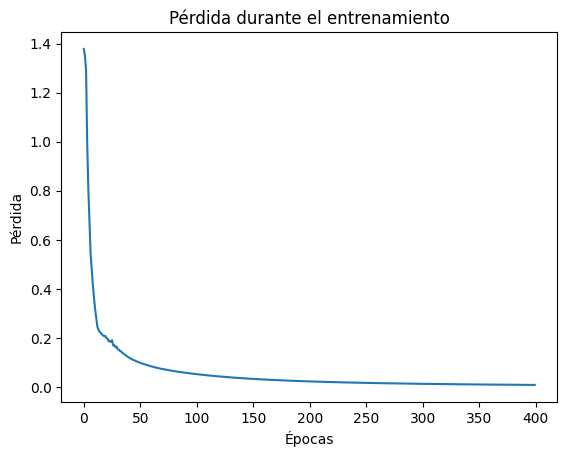
\includegraphics[width=0.8\textwidth]{img/loss}
        \caption{Gráfica de la pérdida durante el entrenamiento}
        \label{fig:plot_loss}
    \end{figure}
    \clearpage

    \subsection{Precisión de los datos de entrenamiento y prueba}\label{subsec:presicion-de-los-datos-de-entrenamiento-y-prueba}
    Para comparar la precisión de los datos de entrenamiento y prueba se invocó el método predict de la red neuronal model con los conjuntos de entrenamiento y prueba.
    Se calcularon el número de predicciones correctas comparando las predicciones con las etiquetas reales.
    Se calculó la precisión como un porcentaje con dos cifras decimales y se imprimió el resultado.
    \begin{lstlisting}[language=Python, caption={Presición de los datos de entrenamiento y prueba}, label={lst:presicion}]
# Realizamos las predicciones para los conjuntos de entrenamiento y prueba
predicciones_entrenamiento = model.predict(X_train)
predicciones_prueba = model.predict(X_test)

# Calculamos el número de predicciones correctas
correctas_entrenamiento = sum(pred == y for pred, y in zip(predicciones_entrenamiento, Y_train))
correctas_prueba = sum(pred == y for pred, y in zip(predicciones_prueba, Y_test))

# Calculamos la precisión como un porcentaje con dos cifras decimales
precision_entrenamiento = round((correctas_entrenamiento / len(Y_train)) * 100, 2)
precision_prueba = round((correctas_prueba / len(Y_test)) * 100, 2)

print(f'Precisión en el conjunto de entrenamiento: {precision_entrenamiento}%')
print(f'Precisión en el conjunto de prueba: {precision_prueba}%')
    \end{lstlisting}
    Al ejecutar el código se obtuvo el siguiente resultado:
    \begin{itemize}
        \item Precisión en el conjunto de entrenamiento: 99.78\%
        \item Precisión en el conjunto de prueba: 87.0\%
    \end{itemize}

    \subsection{Errores de clasificación}\label{subsec:errores-de-clasificacion}
    Para validar visualmente las predicciones de la red neuronal se visualizaron algunas imágenes
    de prueba aleatoriamente con sus predicciones y etiquetas reales.
    \begin{lstlisting}[language=Python, caption={Errores de clasificación}, label={lst:errores_clasificacion}]
# elegir un índice aleatorio y prededir la imagen con el modelo entrenado
import random
n = random.randint(0, 99)
visualize_image(X_test, Y_test, n)

randon_image = X_test[n]
# Realizamos la predicción
prediction = model.predict(randon_image)
print(f'Predicción: {prediction[0]}')
    \end{lstlisting}
    \clearpage
    \noindent
    En algunos casos se puede observar que la red neuronal no clasificó correctamente la imagen.
    Pero teniendo en cuenta que la caligrafía de los dígitos no fue muy buena en esos casos hasta un humano podría tener dificultades para clasificarlos.
    \begin{figure}[!ht]
        \begin{subfigure}
            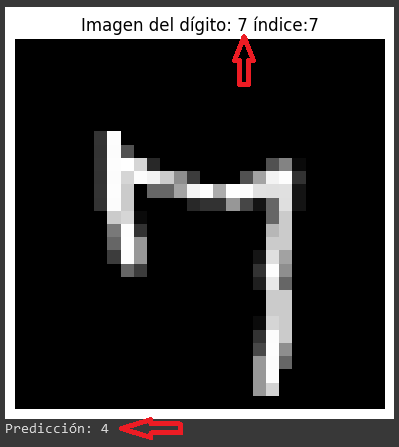
\includegraphics[width=0.5\textwidth]{img/74}\label{fig:74}
        \end{subfigure}
        \begin{subfigure}
            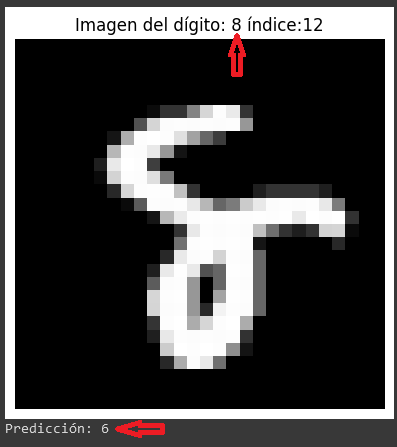
\includegraphics[width=0.5\textwidth]{img/86}\label{fig:86}
        \end{subfigure}
        \begin{subfigure}
            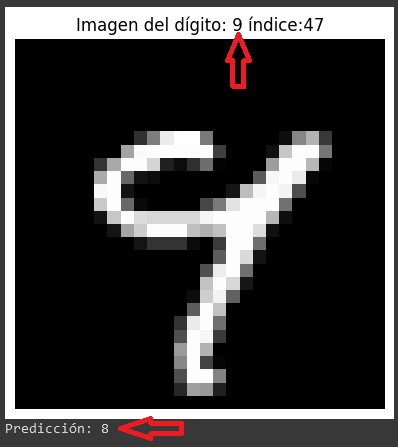
\includegraphics[width=0.5\textwidth]{img/98}\label{fig:98}
        \end{subfigure}
        \begin{subfigure}
            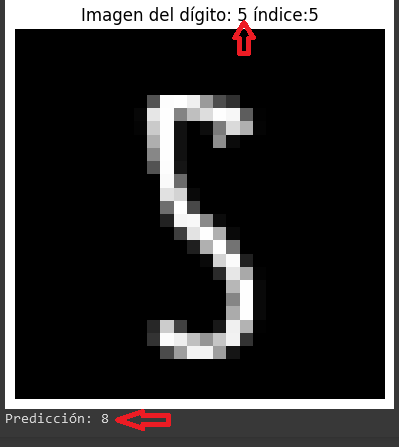
\includegraphics[width=0.5\textwidth]{img/58}\label{fig:58}
        \end{subfigure}
    \end{figure}
    \clearpage


    \section{Conclusiones}\label{sec:conclusiones}
    \noindent
    En este informe se presentó el trabajo realizado en el laboratorio 4 de Redes Neuronales Convolucionales.
    Se implementó una red neuronal artificial multiclase de retropropagación para clasificar imágenes de dígitos escritos a mano.
    La red neuronal implementada consta de 3 capas, una capa de entrada, una capa oculta y una capa de salida.
    La capa de entrada consta de 784 neuronas, una por cada pixel de la imagen.
    La capa oculta consta de 300 neuronas y la capa de salida consta de 10 neuronas, una por cada clase.
    La función de activación utilizada para las neuronas de la capa oculta es la función de activación sigmoide.
    La taza de aprendizaje utilizada es de 0.001 y el número de épocas es de 400.
    La función de costo utilizada es la función de costo de entropía cruzada.
    La actualización de los pesos se realiza utilizando el algoritmo de retropropagación.
    La red neuronal se entrenó utilizando las primeras 900 imágenes y se probó con las 100 restantes.
    Se obtuvo una precisión del 99.78\% en el conjunto de entrenamiento y del 87.0\% en el conjunto de prueba.
    Se visualizaron algunas imágenes de prueba aleatoriamente con sus predicciones y etiquetas reales.
    En algunos casos se observó que la red neuronal no clasificó correctamente la imagen.
    Pero en general, la red neuronal logró clasificar correctamente la mayoría de las imágenes de prueba y entrenamiento.
    Este tipo de herramientas son muy útiles para clasificar imágenes y se pueden utilizar en aplicaciones del mundo real como sistemas de reconocimiento de caracteres,
    sistemas de reconocimiento de voz, sistemas de reconocimiento de objetos, entre otros.

\end{document}
